\section{Verification and paired performance measurements}
\label{sec:experiments}

The experiments separate four questions: whether the new scheduler preserves
the old computation, whether weighted replay returns the correct orbit
partition statistics, whether the geometric weight construction measures
actual surface components, and how much time the implementations consume.
Proofs establish the general claims; these tests check their concrete
realization and expose performance costs that asymptotic analysis omits.

\subsection{Scheduler and repository regression checks}

The scheduler tests compare the complete ordered output and operation trace
against the literal restart implementation, exercise both periodic rules,
check the quadratic allowance, and test cancellation during queue work.
Dedicated cases cover a successful first candidate, a failed first candidate
followed by later successes, and nonperiodic rows interspersed among periodic
ones.  A structural test checks that 256 immediate first-pair mergers read
only linearly many eligibility flags along the new fast path.

The final full repository suite passes 1,047 tests.  It includes all new
weighted and geometric tests and the project's historical independent
oracles.  Nineteen archived Python/license files required by existing tests
were restored from the pinned commit; they are included in the standalone
package.  Their absence in an initially incomplete local snapshot caused
import failures, not a mathematical test failure.  The final recorded log is
\path{results/final_full_tests.log}; it concerns the delivered source.
The suite also prints 13,846 existing expanded-sheet topology comparisons
and 196,712 existing marked-cover comparisons.  Those are inherited coverage,
not newly developed evidence for the component-weight theorem.

\subsection{An independent finite oracle for weighted replay}

For small universes, a literal disjoint-set union structure computes the
entire equivalence relation by expanding every pairing.  Summing the original
weights over its components gives a direct oracle unrelated to interval
reduction.  The new tests compare 660 exhaustive single-generator systems,
2,068 exhaustive ordered two-generator systems, and 3,000 randomized signed
systems under each of the two periodic rules.  Two additional targeted
finite comparisons bring the total to 8,730 profile comparisons.

The exhaustive tests use basis-vector weights: the sum on an orbit identifies
its complete set of points, so they test the partition rather than only
coarse counts.  The randomized tests use signed vector fields, reflections,
translations, static gaps, and adjacent coalescing runs.  Across the finite
comparisons, 28,656 full-range transfers are observed, including 13,988
periodic transfers before partial truncations.  All six local-operation
types occur.  The largest observed increase in maximal runs is three,
consistent with the proved upper bound of four.

Separate nonexpanding cases use universe sizes with 65,537 bits and weight
entries with 8,192 bits.  They check uniform periodic, reflection, and static
systems, signed hexadecimal transport, malformed partitions, zero weights,
cycle caps, and callback exceptions.  These large-bit cases test dependence
on encoding length; they do not use literal component expansion as an oracle.
Their expected profiles are computed from simple closed formulas.

\subsection{Independent normal-surface component comparisons}

The geometric audit compares three views of each finite input: literal
connectivity of the original normal-arc point graph with cellular weight
sums, the production compressed profile, and actual connected normal-surface
components returned by Regina 7.4 \cite{Regina}.  The last comparison checks
Euler characteristic, polygon counts, boundary edge weights, cycle-support
intersection counts, and disk predicates.  Thus it does not merely compare
two calls that share the new Euler-weight formula.

The fixed audit contains 237 cases:
\begin{center}
\begin{tabular}{lr}
\toprule
Family & Cases \\
\midrule
Layered meridians with 1--6 tetrahedra and scales 0--3 & 24 \\
Vertex normal surfaces after 0--3 boundary caps & 134 \\
Sphere/disk/M\"obius mixtures, coefficients 0--3 & 64 \\
Vertex normal surfaces of a fixed finite trefoil exterior & 15 \\
\midrule
Total, with no mismatches & 237 \\
\bottomrule
\end{tabular}
\end{center}
The finite trefoil triangulation and its 15 vectors are frozen as JSON; the
audit does not depend on reproducing a heuristic simplification sequence.
It has five tetrahedra and isomorphism signature
\texttt{fLHPccdeeeqcieh}.  The audit is a supplied-surface comparison, not a
claim that a general knot-recognition benchmark has been run.

The dependency-free demonstration makes the semantic gain visible.  In a
one-tetrahedron solid torus, a meridian plus a boundary vertex-link has
coordinate gcd one, two components, two disks, and one compressing disk.
The two component vectors have Euler characteristic one but different
boundary parity.  A second input consists of $2^{5000}$ parallel meridian
disks and returns one profile group with a 5,001-bit multiplicity.
Its serialized certificate occupies 37,637 bytes in this fixture, rather
than one record per disk.  Both examples verify before and after the
hexadecimal JSON round trip.  The concise output is included as
\path{results/component_demo.json}.

These finite oracles do not replace the proofs.  In particular, they cannot
establish a global AHT trace bound, completeness of a surface search, or
soundness of a missing diagram-to-exterior construction.

\subsection{Timing protocol}

All final timings use CPython 3.12.14 on an x86-64 Linux environment.  Each
case has seven paired rounds; arm order is independently shuffled with seed
26100945.  The comparison loads the actual pinned
\path{interval_orbits.py} as a separate baseline module, rather than treating
the new program's \code{legacy} wrapper as its historical implementation.
Input pairings are preconstructed immutable objects of the appropriate
module type.  Timing covers a complete orbit count with certificate
recording disabled.

Before timing each case, complete certificates from the old, adaptive, and
eager-queue arms are compared for exact equality and checked with the
independent verifier.  All 19 cases pass this stronger trace test.
There are 399 recorded orbit timings, 70 native topology-query timings,
and 67 excluded warmups.  Heavy regression and oracle jobs were not run
concurrently with these measurements.  Raw samples, parameters, counters,
and medians are retained in \path{results/benchmark_orbits.json}.

Tables report elapsed-time medians.  A paired gain is the median of seven
old/adaptive ratios; it need not equal the ratio of the separately reported
time medians.  Seven rounds on one environment characterize this run, not
a hardware-independent constant or a statistical claim about all inputs.
Exact operation counts and the proved family bounds provide the asymptotic
evidence; timing curves are supporting implementation evidence.

\subsection{The complete five-cycle family}

\Cref{tab:five-cycle} reports the family proved in
\cref{sec:queue}.  At $k=256$, the old implementation performs 2,105,660
merger tests, the eager queue 81,154, and the adaptive path 97,409.
All three execute exactly five cycles and return one orbit.  Median
complete-count time falls from 1,824.929 ms to 118.591 ms for the adaptive
path; the median paired gain is 15.56.  There is one adaptive queue switch
in each family member.

\begin{table}[htbp]
\centering
\small
\begin{tabular}{rrrrrrr}
\toprule
$k$ & Old tests & Queue tests & Old ms & Adaptive ms & Queue ms & Paired gain \\
\midrule
16 & 560 & 274 & 0.572 & 0.429 & 0.455 & 1.34 \\
32 & 4,260 & 1,186 & 3.809 & 1.659 & 1.769 & 2.27 \\
64 & 33,356 & 4,930 & 30.147 & 7.135 & 7.207 & 4.27 \\
128 & 264,348 & 20,098 & 240.448 & 28.229 & 29.778 & 8.32 \\
256 & 2,105,660 & 81,154 & 1824.929 & 118.591 & 125.524 & 15.56 \\
\bottomrule
\end{tabular}
\caption{Complete five-cycle counts: exact merger tests and median elapsed times.}
\label{tab:five-cycle}
\par\smallskip\footnotesize Paired gain is the median of the seven old/adaptive time ratios; it need not equal the ratio of the two medians. All cases have five cycles.
\end{table}

\begin{figure}[htbp]
\centering
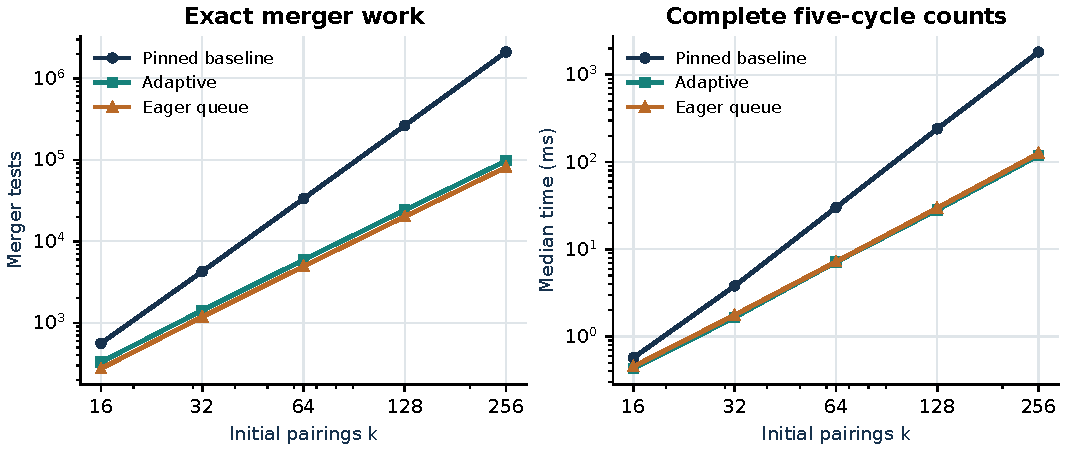
\includegraphics[width=\textwidth]{figures/five_cycle.pdf}
\caption{Exact merger work and complete-count time on the proved family.
Both axes are logarithmic. The curves illustrate the cubic versus quadratic
merger counts; the exponent claim comes from the proof, not curve fitting.}
\label{fig:five-cycle}
\end{figure}

Increasing the translation base to create longer integers leaves the
combinatorial trace pattern unchanged.  At 32 pairings and 66, 1,026, or
4,098 bits for $N$, all cases still take five cycles, with 4,260 old tests,
1,425 adaptive tests, and 1,186 eager tests.  The adaptive paired gains are
2.35, 2.64, and 2.72 respectively; arithmetic is included in elapsed time.
\begin{table}[htbp]
\centering
\small
\begin{tabular}{rrrrr}
\toprule
Bits of $N$ & Old ms & Adaptive ms & Queue ms & Paired gain \\
\midrule
66 & 4.721 & 2.003 & 2.019 & 2.35 \\
1026 & 7.401 & 2.814 & 2.669 & 2.64 \\
4098 & 16.278 & 5.989 & 5.245 & 2.72 \\
\bottomrule
\end{tabular}
\caption{Fixed 32-pairing, five-cycle instances with increasing endpoint bit length.}
\label{tab:binary}
\end{table}


\subsection{Easy inputs and native geometry}

An eager queue can be expensive when the first available pair always merges.
It evaluates $(k-1)^2$ candidates where the restart scan needs only $k-1$.
At 256 duplicate pairings, its median is 189.053 ms versus 1.109 ms for the
baseline.  This is why queue mode is an experimental option and the bounded
adaptive policy is the default.

An initial adaptive implementation also rebuilt the full periodic index
list after every immediate success.  Profiling exposed that avoidable cost
and motivated the lazy first-pair path in the delivered implementation.
The final easy-input measurements in \cref{tab:easy} place the adaptive
path close to the baseline; paired gains range from 0.945 to 1.022 across
the four cases.  A gain below one is a measured slowdown.  The new default
does not promise universal speedup.
\begin{table}[htbp]
\centering
\small
\begin{tabular}{rrrrrr}
\toprule
$k$ & Tests: old/adaptive & Old ms & Adaptive ms & Queue ms & Paired gain \\
\midrule
16 & 15 & 0.072 & 0.074 & 0.561 & 0.98 \\
64 & 63 & 0.275 & 0.287 & 9.916 & 0.96 \\
128 & 127 & 0.572 & 0.570 & 42.696 & 1.02 \\
256 & 255 & 1.109 & 1.131 & 189.053 & 0.94 \\
\bottomrule
\end{tabular}
\caption{Easy duplicate inputs. All adaptive runs complete without a queue switch.}
\label{tab:easy}
\end{table}


For native geometry, layered solid-torus meridian systems range from 4 to
128 tetrahedra.  Their normal coordinates and interval endpoints grow in
binary size with the layering.  The adaptive path performs exactly the
same number of merger tests as the old implementation and never switches
to the queue.  Its gain comes from indexing periodic rows once after a
failed first pair and avoiding repeated inner visits to nonperiodic rows.
At 128 tetrahedra, the median paired gain is 1.51, with median times
886.982 ms and 593.443 ms.  The smallest case is slightly slower.
\begin{table}[htbp]
\centering
\small
\begin{tabular}{rrrrrrr}
\toprule
$t$ & $k$ & Bits of $N$ & Cycles & Old ms & Adaptive ms & Paired gain \\
\midrule
4 & 18 & 6 & 9 & 0.337 & 0.339 & 0.97 \\
8 & 34 & 8 & 13 & 0.978 & 0.952 & 1.03 \\
16 & 66 & 14 & 21 & 4.365 & 3.932 & 1.11 \\
32 & 130 & 25 & 37 & 21.056 & 17.369 & 1.22 \\
64 & 258 & 47 & 69 & 130.881 & 95.281 & 1.35 \\
96 & 386 & 69 & 101 & 388.928 & 267.030 & 1.44 \\
128 & 514 & 92 & 133 & 886.982 & 593.443 & 1.51 \\
\bottomrule
\end{tabular}
\caption{Complete interval counts on native layered-solid-torus meridian arc systems.}
\label{tab:native}
\par\smallskip\footnotesize Geometry is constructed before timing. There are no adaptive queue switches and no changes in merger-test count in these cases.
\end{table}

\begin{figure}[htbp]
\centering
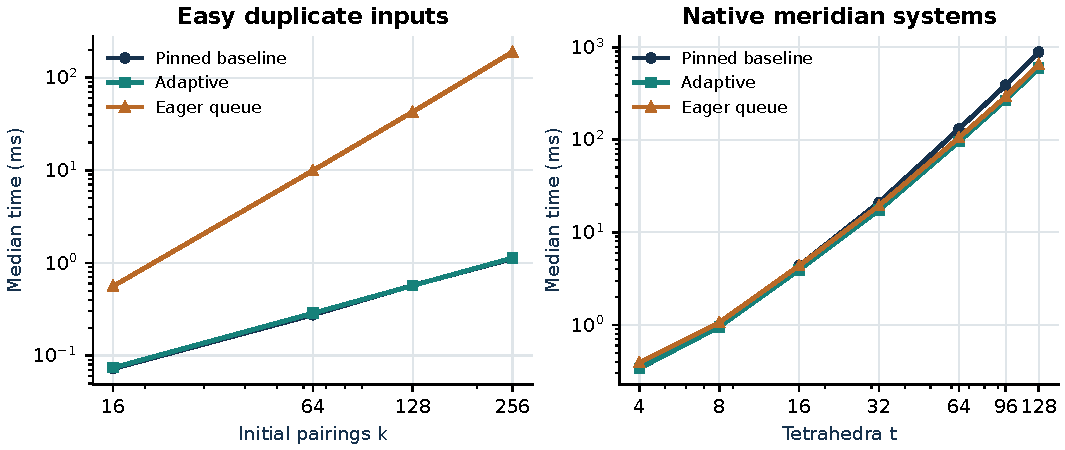
\includegraphics[width=\textwidth]{figures/easy_and_native.pdf}
\caption{The adaptive policy avoids the eager queue's large easy-input
cost. Native meridian systems show more modest gains without a queue switch.
Both axes are logarithmic; these are separate input families.}
\label{fig:easy-native}
\end{figure}

Finally, \cref{tab:profile-costs} records whole native queries, including
fresh geometry validation, for the established aggregate topology interface
and the new five-coordinate component profile.  The new interface obtains
its disk predicates from one weighted orbit calculation and needs no
orientation-double query.  At 96 tetrahedra the observed medians are
547.781 ms and 359.843 ms.  The output contracts differ, so this is a cost
comparison rather than a same-task speedup claim.  It shows that the richer
component information is practical on these fixtures; it does not measure
the time required to discover a useful normal surface.
\begin{table}[htbp]
\centering
\small
\begin{tabular}{rrr}
\toprule
$t$ & Aggregate topology ms & Component profile ms \\
\midrule
4 & 1.183 & 1.182 \\
16 & 9.806 & 8.132 \\
32 & 38.328 & 29.382 \\
64 & 195.910 & 137.648 \\
96 & 547.781 & 359.843 \\
\bottomrule
\end{tabular}
\caption{Native query costs, including fresh geometry validation. The outputs differ.}
\label{tab:profile-costs}
\par\smallskip\footnotesize These are costs of two different interfaces, not a same-task speedup experiment.
\end{table}


\subsection{What the measurements support}

The strongest supported performance conclusion is the proved improvement
for complete counts on the explicit interval family.  The native cases
support a smaller practical gain and validate the geometry-to-orbit path.
The component audit supports the implementation of the new certificate
predicate, and the huge-multiplicity demo confirms that its interface stays
compressed.  No experiment here measures a complete new knot recognizer on
hard diagrams, and none establishes the candidate or hierarchy bounds
required for the quasi-polynomial objective.
